\chapter{블랙홀 엔트로피, 홀로그래피, 드시터르 공간}

\lectureoverview{앞선 강의에서 시작한 대응 논증을 마무리한다. 고도로 여기된 끈의 엔트로피는 질량에 비례하는 반면, 슈바르츠실트 블랙홀의 엔트로피는 면적에 비례한다. 두 식은 강한 중력장을 가진 블랙홀을 자유 끈과 동일시해서 연결되는 것이 아니라, 끈 결합상수를 천천히 변화시켜 두 기술 방식이 만나는 지점에 이르러 연결된다. 그러면 면적 법칙은 자연스럽게 홀로그래피 원리로 이어진다. 강의의 마지막 부분에서는 팽창하는 공간과 드시터르 기하를 소개한다. 그 지평선은 다음 강의에서 살펴본다.}

\section{계수 문제로 돌아가기}

긴 끈의 개수를 셀 때 아직 매듭짓지 않은 문제가 하나 있었다. 고정된 총길이를 여러 끈에 나누어 배정하면, 길이가 같은 동일한 끈들은 서로 구별되지 않는다. 하지만 상자 안에서 끈이 차지하는 위치는 상태의 일부이며, 상자의 크기는 해당하는 하나의 긴 끈이 차지하는 영역과 대략 같게 정한다.

\begin{classroomqa}
\audiencequestion{짧은 끈들은 서로 구별되는가? 끈들의 위치도 계산에 포함되는가?\lecturetimestamp{00:00:37}}
\lecturerresponse{성질이 동일한 끈들은 서로 구별되지 않지만, 상자 안에서 끈들이 차지하는 위치는 계산에 포함한다. 부피를 고정한 채 비교하며, 그 부피는 긴 끈이 차지하는 영역과 같게 정한다.}
\end{classroomqa}

이 문제를 정리했으니 이제 목표를 말할 수 있다. 몇 가지 방정식을 모아 블랙홀 엔트로피의 스케일링을 구할 것이다. 적분이나 무한합은 필요하지 않다. 어려움은 대수 계산에 있지 않다. 어떤 양들을 서로 비교할 수 있는지, 논증의 어느 단계에서 비교해야 하는지를 아는 데 있다.

\section{자연 단위계와 플랑크 면적}

다음과 같이 두되
\begin{equation}
c=\hbar=1,
\label{eq:l07-natural-units}
\end{equation}
뉴턴 상수는 명시적으로 남겨 둔다. 우선 시간과 길이의 단위가 같아진다. 광자 관계식
\begin{equation}
E=\frac{\hbar c}{\lambda}
\end{equation}
과 질량-에너지 관계식 \(E=mc^2\)에서 다음을 얻는다.
\begin{equation}
[M]=L^{-1}.
\label{eq:l07-mass-dimension}
\end{equation}
따라서 질량은 역길이 단위로 나타낼 수 있다.

\begin{figure}[htbp]
\centering
\includegraphics[width=0.62\textwidth]{lecture_07_figure_02.png}
\caption{차원 논증을 시작할 때 사용하는 자연 단위계 관례. 에너지 식은 위 방정식들에서 완성된다.}
\lectureframe{00:03:27.900}
\end{figure}

\(G_N\)의 단위를 정하려면 뉴턴 역학의 가속도를 차원 계산에만 사용한다.
\begin{equation}
a\sim\frac{G_NM}{R^2}.
\end{equation}
\(T\)과 \(L\)의 단위가 같으므로 \([a]=L/T^2=L^{-1}\)이다. 이를 식~\eqref{eq:l07-mass-dimension}과 함께 사용하면 다음을 얻는다.
\begin{equation}
[G_N]=L^2.
\end{equation}
이 단위계에서 뉴턴 상수는 면적이다. 플랑크 길이를
\begin{equation}
G_N=\ell_p^2,
\label{eq:l07-planck-area}
\end{equation}
로 정의하면, \(A/G_N=A/\ell_p^2\)가 무차원인 이유를 곧바로 알 수 있다. 이는 플랑크 면적 단위로 면적을 잰 값이다.

\section{끈 결합상수와 중력의 세기}

이제 중력을 끈 이론의 언어로 바꾸어야 한다. 유용한 그림은 교환 과정이다. 끈이 자기 자신과 교차할 때 분열한 뒤 다시 결합할 수 있다. 한 물체가 작은 닫힌 끈 고리를 방출하고 다른 물체가 이를 흡수할 수 있다. 그 들뜸이 중력자라면 이 과정이 중력을 매개한다. 방출 때 한 번, 흡수 때 한 번 상호작용 인자가 나타나므로 교환 세기에는 \(g_s^2\)가 포함된다.

결합상수 \(g_s\)는 무차원이다. 더 정확히 말하면 진폭 수준의 결합상수이며, 확률이나 율은 \(g_s^2\) 차수에서 시작한다.\editorialnote{강의에서는 때때로 \(g_s\)를 확률이라고 부른 뒤 확률의 제곱근이라고 정정한다. 섭동 결합상수는 진폭 수준의 양이다.} \(G_N\)은 면적의 차원을 가지므로 길이 척도가 여전히 필요하다. 기본 끈 길이 \(\ell_s\)는 기본적인 끈 요동 하나의 척도이며, 필요한 길이 척도를 제공한다.
\begin{equation}
G_N\sim g_s^2\ell_s^2,
\qquad
\ell_p\sim g_s\ell_s.
\label{eq:l07-planck-string}
\end{equation}

\begin{figure}[htbp]
\centering
\includegraphics[width=0.72\textwidth]{lecture_07_figure_05.png}
\caption{칠판에 적힌 결합상수 관계: \(G_N=\ell_p^2\)와 \(g_s^2\ell_s^2\sim\ell_p^2\).}
\lectureframe{00:12:15.000}
\end{figure}

약한 결합에서 \(g_s\ll1\)이면 플랑크 길이는 끈 길이보다 훨씬 짧다. \(g_s\)를 낮추면 기본 끈의 척도는 고정한 채 중력이 약해진다.\editorialnote{유효 4차원 이론에서는 압축화 자료와 수치 관례도 \(G_N\)에 들어간다. 이 스케일링 논증에서는 이를 고정하고 생략한다.}

\section{긴 끈의 계수}

엔트로피는 상태를 지정하는 데 필요한 기본 선택의 수를 센다. 고도로 여기된 끈을 정사각 격자 위의 보행으로 바꾸어 생각해 보자. 각 꼭짓점에서 다음 링크는 네 방향 가운데 하나를 향할 수 있다. 기본 선택을 네 가지 중 하나를 고르는 것으로 보든, 두 번의 이진 선택으로 보든 달라지는 것은 1 정도의 상수뿐이다. 중요한 것은 걸음의 수다.

\(L\)가 끈의 윤곽 길이이고 각 걸음의 길이가 \(\ell_s\)라면
\begin{equation}
N=\frac{L}{\ell_s}
\end{equation}
걸음이 필요하다. 보행의 수는 개략적으로 \(\Omega_N\sim q^N\)처럼 지수적으로 증가하며, \(q\)는 1 정도의 값이다. 따라서
\begin{equation}
S_{\mathrm{str}}=\log\Omega_N\sim N\sim\frac{L}{\ell_s}.
\label{eq:l07-string-entropy-length}
\end{equation}

\begin{figure}[htbp]
\centering
\includegraphics[width=0.68\textwidth]{lecture_07_figure_03.png}

\vspace{0.7em}
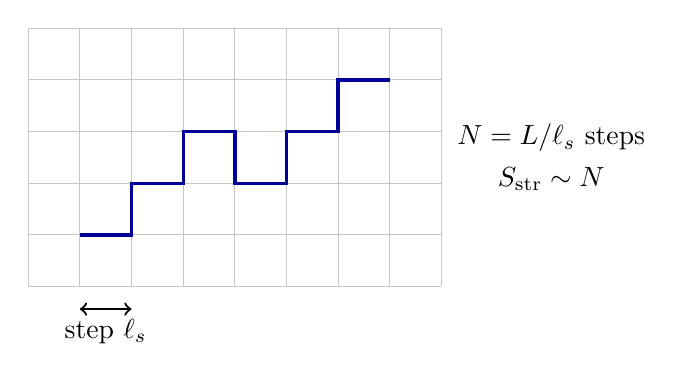
\begin{tikzpicture}[scale=0.82]
  \draw[step=0.8cm,gray!45,thin] (0,0) grid (6.4,4.0);
  \draw[very thick,blue!60!black]
    (0.8,0.8)--(1.6,0.8)--(1.6,1.6)--(2.4,1.6)--(2.4,2.4)--
    (3.2,2.4)--(3.2,1.6)--(4.0,1.6)--(4.0,2.4)--(4.8,2.4)--
    (4.8,3.2)--(5.6,3.2);
  \draw[<->,thick] (0.8,-0.35)--(1.6,-0.35);
  \node[below] at (1.2,-0.35) {step \(\ell_s\)};
  \node[align=center] at (8.1,2.0) {\(N=L/\ell_s\) steps\\[0.3em]\(S_{\mathrm{str}}\sim N\)};
\end{tikzpicture}
\caption{칠판의 격자 모형과 이를 정리한 무작위 보행 해석. 엉킨 공의 지름이 아니라 윤곽 길이가 선택의 수를 결정한다.}
\lectureframe{00:17:20.000}
\end{figure}

같은 기본 선분들로 질량을 센다. 길이 \(\ell_s\)인 선분의 질량 척도는
\begin{equation}
m_{\mathrm{seg}}\sim\frac{1}{\ell_s}.
\end{equation}

\begin{classroomqa}
\audiencequestion{기본 선분에 길이 \(\ell_s\)를 부여하는 건가요?\lecturetimestamp{00:18:56}}
\lecturerresponse{그렇다. 그 특성 길이는 \(\ell_s\)이므로 자연 단위계에서 특성 질량은 \(1/\ell_s\)이다.}
\end{classroomqa}

\(L/\ell_s\)개의 선분 질량을 더하면 다음과 같다.
\begin{equation}
M\sim\frac{L}{\ell_s}\frac{1}{\ell_s}
=\frac{L}{\ell_s^2},
\qquad
L\sim M\ell_s^2.
\label{eq:l07-string-mass}
\end{equation}
진동하는 끈의 운동에너지와 퍼텐셜 에너지는 이 스케일링 관계에 압축되어 있다. 상세한 통계역학적 처리를 해도 같은 의존성을 얻는다. 식~\eqref{eq:l07-string-entropy-length}에 대입하면 필요한 끈 이론의 식을 얻는다.
\begin{equation}
S_{\mathrm{str}}\sim M\ell_s.
\label{eq:l07-string-entropy-mass}
\end{equation}

\begin{figure}[htbp]
\centering
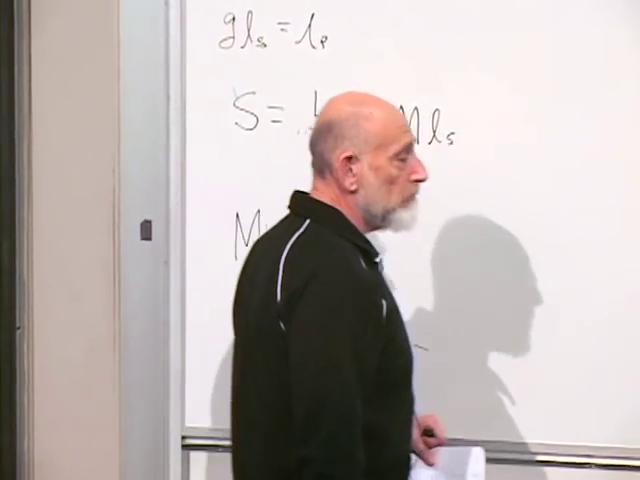
\includegraphics[width=0.66\textwidth]{lecture_07_figure_04.png}
\caption{비교에 앞서 정리한 끈 이론 쪽의 항목: \(\ell_p\sim g_s\ell_s\), \(S_{\mathrm{str}}\sim L/\ell_s\sim M\ell_s\), \(M\sim L/\ell_s^2\).}
\lectureframe{00:21:57.800}
\end{figure}

\section{자유 끈이 아직 블랙홀이 아닌 이유}

중력 쪽의 정확한 반고전적 공식은 다음과 같다.
\begin{equation}
S_{\mathrm{BH}}=\frac{A}{4G_N}.
\label{eq:l07-bh-exact}
\end{equation}

\begin{classroomqa}
\audiencequestion{분모에 들어가는 수치 계수는 얼마인가요?\lecturetimestamp{00:23:28}}
\lecturerresponse{4이다. 대응 논증으로 스케일링은 얻을 수 있지만, 이 논증은 너무 거칠어서 정확한 계수를 결정할 수 없다.}
\end{classroomqa}

4차원 슈바르츠실트 블랙홀에서는
\begin{equation}
R_s=2G_NM,
\qquad
A=4\pi R_s^2.
\end{equation}
강의에서처럼 수치 상수를 생략하면
\begin{align}
S_{\mathrm{BH}}
&\sim\frac{A}{G_N}
\sim\frac{(G_NM)^2}{G_N} \\
&\sim M^2G_N
\sim M^2\ell_p^2.
\label{eq:l07-bh-scaling}
\end{align}

\begin{figure}[htbp]
\centering
\includegraphics[width=0.72\textwidth]{lecture_07_figure_06.png}
\caption{칠판에서 완성한 비교: 끈 엔트로피는 끈 단위의 길이인 반면, 블랙홀 엔트로피는 플랑크 단위의 면적이다.}
\lectureframe{00:25:35.000}
\end{figure}

식~\eqref{eq:l07-string-entropy-mass}와 \eqref{eq:l07-bh-scaling}의 유사성은 시사하는 바가 있지만, 두 식은 같지 않다. 원래 블랙홀을 자유 끈이라고 부르고 대입하는 것은 잘못이다. 자유 끈의 계수에서는 끈을 이루는 부분들 사이의 인력이 빠져 있다. 바로 그 상호작용이 끈을 블랙홀 크기로 압축하고 음의 결합에너지를 통해 전체 에너지를 낮춘다.

별을 보면 이 오류가 익숙한 형태로 드러난다. 별의 질량을 가진 뜨거운 기체를 지나치게 큰 상자에 넣어 두는 것은 온도가 같더라도 별의 모형이 아니다. 자체 중력은 평형 크기와 에너지-엔트로피 관계를 바꾼다. 긴 끈의 모든 자체 상호작용을 따라가는 일은 어려우므로 그렇게 하지 않을 것이다.

\begin{classroomqa}
\audiencequestion{긴 끈에서 작은 고리가 떨어져 나가면 엔트로피가 감소합니다. 그렇다면 중력자 교환은 중력계의 엔트로피를 낮추나요?\lecturetimestamp{00:28:48}}
\lecturerresponse{여기서 다루는 평형 교환 과정에서는 그렇지 않다. 가상 들뜸은 양방향으로 방출되고 흡수된다. 이 그림은 끈 조각이 영구적으로 떨어져 나가는 실제 상황을 나타내지 않는다. 지금 이 그림의 목적은 결합상수 인자가 두 개 나타난다는 점과 그에 따라 \(g_s^2\) 의존성이 생긴다는 점만 보이는 것이다.}
\end{classroomqa}

\section{단열 대응 논증}

중력이 무시되는 조건에서 시작하자. \(g_s\to0\)일 때 끈들은 서로 지나쳐 가며 분열하거나 결합하지 않고, 자체 중력에 의한 인력도 사라진다. \(g_s\)를 높이면서 \(\ell_s\)는 고정하면 중력이 강해지고, 고도로 여기된 끈은 수축하다가 결국 블랙홀이 된다. 조절 변수를 천천히 되돌리면 블랙홀은 끈 상태로 돌아와야 한다. 긴 끈 몇 개가 될 수도 있지만, 앞선 강의의 고에너지 상태 수 계산에 따르면 지배적인 부문에는 짧은 끈으로 이루어진 엄청난 기체가 아니라 긴 끈 하나가 들어 있다.

\begin{classroomqa}
\audiencequestion{결합상수를 바꾸는 동안 무엇을 고정하나요?\lecturetimestamp{00:32:19}}
\lecturerresponse{끈 길이 \(\ell_s\), 따라서 기본 끈의 질량 척도 \(1/\ell_s\)를 고정한다. 조절 변수는 \(g_s\)를 바꾸고, 그에 따라 \(G_N\sim g_s^2\ell_s^2\)도 바뀐다.}
\end{classroomqa}

변화는 느리고 고립된 가역 과정이어야 한다. 이 조건에서는 엔트로피가 단열 불변량이다.
\begin{equation}
\Delta S=0.
\label{eq:l07-adiabatic}
\end{equation}
소산이나 통제되지 않은 천이가 일어난다면 느리게 변화시키는 것만으로는 충분하지 않다. 여기서 ``단열''이란 같은 상태들의 계열을 연속적으로 따라갈 수 있다는 뜻이다.\editorialnote{이는 가역적인 열역학 과정에서 말하는 단열의 의미다. 비가역 과정은 열의 출입이 없다는 의미에서는 단열이어도 엔트로피를 생성할 수 있다.}

목표 블랙홀의 질량을 \(M_0\), 결합상수를 \(g_{s,0}\)라고 하자. 설명하려는 면적 공식을 쓰기 전에 차원 분석으로 말할 수 있는 것은 중성 비회전 블랙홀의 엔트로피가 무차원 조합의 어떤 함수라는 점뿐이다.
\begin{equation}
S_{\mathrm{BH}}=f(M\ell_p)
=f(Mg_s\ell_s).
\label{eq:l07-entropy-function}
\end{equation}
\(\ell_s\)를 고정하면 등엔트로피 경로에서는 따라서 다음 양이 일정하게 유지된다.
\begin{equation}
Mg_s=M_0g_{s,0}
\label{eq:l07-adiabat}
\end{equation}
단, 같은 상태 가지를 따라간다고 가정한다.

\(g_s\)가 감소하면 음의 결합에너지가 제거되므로 이 경로를 따라 질량 \(M\)는 증가한다. 바탕이 되는 끈 구성도 결합이 느슨해져 퍼진다. 그러나 형식적인 슈바르츠실트 반지름은 단열 경로에서 \(R_s\sim Mg_s^2\ell_s^2\sim g_s\ell_s\)처럼 변하므로 감소한다.\editorialnote{구어 설명에서는 중력에 의한 결합에서 풀려난 물체에 대해 ``커진다''고 말한다. 이를 유도된 단열 경로를 따라 슈바르츠실트 반지름이 커진다는 뜻으로 받아들여서는 안 된다.}

\begin{classroomqa}
\audiencequestion{중력이 약해지면 물체는 커지나요, 작아지나요?\lecturetimestamp{00:36:28}}
\lecturerresponse{끈 구조는 결합에서 풀려나 팽창하고, 음의 결합에너지가 제거되므로 질량은 증가한다. 블랙홀 공식으로 정하는 반지름은 끈 척도에 이를 때까지 감소하며, 그 지점에서는 블랙홀 기술 방식이 더 이상 유용하지 않다.}
\end{classroomqa}

\section{두 곡선과 교점}

세로축에 질량, 가로축에 끈 결합상수를 놓고 그린다. 식~\eqref{eq:l07-adiabat}은 쌍곡선 \(M\propto g_s^{-1}\)이다.

\begin{classroomqa}
\audiencequestion{곱 \(Mg_s\)이 일정한 곡선은 어떤 모양인가요?\lecturetimestamp{00:44:08}}
\lecturerresponse{쌍곡선이다. 목표점 \((g_{s,0},M_0)\)을 지나는 단열 곡선이다.}
\end{classroomqa}

두 번째 곡선은 기술 방식이 바뀌는 교차 구간을 나타낸다. 블랙홀의 반지름이 기본 끈 요동의 크기보다 작아지면 이를 통상적인 슈바르츠실트 기하로 분해해 볼 수 없다. 따라서 대응점을 다음과 같이 추정한다.
\begin{equation}
R_s\sim\ell_s.
\label{eq:l07-correspondence-radius}
\end{equation}
\(R_s\sim MG_N\)와 식~\eqref{eq:l07-planck-string}을 사용하면 다음과 같다.
\begin{equation}
Mg_s^2\ell_s^2\sim\ell_s,
\qquad
Mg_s^2\sim\frac{1}{\ell_s}.
\label{eq:l07-transition-curve}
\end{equation}
따라서 전이 곡선은 \(M\propto g_s^{-2}\)에 따라 감소하며, 단열 곡선보다 더 가파르다.

\begin{figure}[htbp]
\centering
\includegraphics[width=0.70\textwidth]{lecture_07_figure_07.png}

\vspace{0.6em}
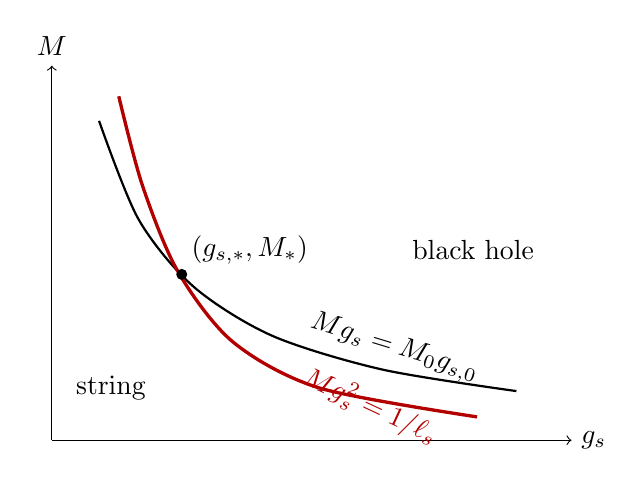
\begin{tikzpicture}[x=1cm,y=0.78cm]
  \draw[->] (0.4,0.4)--(7.0,0.4) node[right] {\(g_s\)};
  \draw[->] (0.4,0.4)--(0.4,6.5) node[above] {\(M\)};
  \draw[thick,black] plot[smooth] coordinates {(1.0,5.6) (1.5,4.0) (2.2,2.9) (3.2,2.1) (4.6,1.55) (6.3,1.2)};
  \draw[very thick,red!70!black] plot[smooth] coordinates {(1.25,6.0) (1.55,4.55) (2.0,3.15) (2.7,2.0) (3.8,1.25) (5.8,0.78)};
  \fill (2.05,3.1) circle (2pt) node[above right] {\((g_{s,*},M_*)\)};
  \node[black,rotate=-17] at (4.75,1.9) {\(Mg_s=M_0g_{s,0}\)};
  \node[red!70!black,rotate=-25] at (4.45,0.95) {\(Mg_s^2=1/\ell_s\)};
  \node at (5.75,3.5) {black hole};
  \node at (1.15,1.25) {string};
\end{tikzpicture}
\caption{칠판의 그래프와 이를 정리한 해석. 검은색 단열 곡선은 더 가파른 빨간색 대응 곡선과 교차한다. 그 교점에서 물체는 끈과 같은 성질을 띠게 된다.}
\lectureframe{00:49:35.000}
\end{figure}

교점 \((M_*,g_{s,*})\)에서는 두 방정식이 다음과 같다.
\begin{align}
M_*g_{s,*} &= M_0g_{s,0}, \\
M_*g_{s,*}^2 &\sim \frac{1}{\ell_s}.
\end{align}
첫 번째 방정식을 제곱하고 두 번째 방정식으로 나누면
\begin{equation}
M_*
\sim M_0^2g_{s,0}^2\ell_s.
\end{equation}
\(\ell_s\)를 곱하면
\begin{equation}
M_*\ell_s
\sim M_0^2g_{s,0}^2\ell_s^2
\sim M_0^2G_{N,0}.
\label{eq:l07-crossover-result}
\end{equation}

\begin{figure}[htbp]
\centering
\includegraphics[width=0.68\textwidth]{lecture_07_figure_08.png}
\caption{\(M_*\ell_s=M_0^2g_{s,0}^2\ell_s^2=M_0^2G_{N,0}\)를 포함해 완성한 교차 구간의 대수 계산.}
\lectureframe{00:54:40.000}
\end{figure}

\begin{classroomqa}
\audiencequestion{두 곡선의 방정식을 나눌 때 \(\ell_s\)는 분자의 위쪽에 오나요, 분모의 아래쪽에 오나요?\lecturetimestamp{00:52:41}}
\lecturerresponse{위쪽에 온다. \(1/\ell_s\)로 나누는 것은 \(\ell_s\)를 곱하는 것이므로 \(M_*\sim M_0^2g_{s,0}^2\ell_s\)가 된다.}
\end{classroomqa}

교차점에서는 끈 이론의 식이 유효하므로
\begin{equation}
S_*\sim M_*\ell_s.
\end{equation}
경로를 따라 엔트로피는 변하지 않았다. 이 사실을 식~\eqref{eq:l07-crossover-result}과 결합하면 원래 목표 블랙홀의 엔트로피를 얻는다.
\begin{equation}
S_{\mathrm{BH}}(M_0)
\sim M_0^2G_{N,0}
\sim M_0^2\ell_{p,0}^2.
\label{eq:l07-final-correspondence}
\end{equation}
이것이 원하는 면적 법칙의 스케일링이다.

\section{대응 논증이 증명하는 것과 증명하지 않는 것}

이 구성은 처음의 강한 중력장을 가진 블랙홀이 자유 끈이라고 말하지 않는다. 물체를 끈의 개수를 신뢰할 수 있는 영역으로 옮겨 그곳에서 엔트로피를 구한 다음, 그 엔트로피를 가역 경로를 따라 원래 상태로 되가져온다. 전이는 뚜렷한 상 경계가 아니라 크로스오버이므로, 이 추정으로는 계수 \(1/4\)를 식~\eqref{eq:l07-bh-exact}에서 정할 수 없다.

같은 논리는 전하를 띤 블랙홀, 다른 차원의 블랙 물체, 확장된 블랙 브레인에도 매개변수 의존성을 따지는 수준에서 성립한다. 대칭성이 더 크고 초대칭인 경우에는 결합상수가 변해도 보호되는 상태 계수를 통해 정확한 정보를 유지할 수 있다. 이런 방법은 수치 계수까지 얻지만, 여기서의 개념적 논증에는 필요하지 않은 수학적 장치를 더한다.

무엇보다 이 계산은 미시적 해석을 제공한다. 엔트로피는 숨겨진 구조의 증거다. 유체역학은 분자를 다루지 않고 밀도, 압력, 흐름을 기술하지만, 유체의 엔트로피는 그런 미시적 자유도가 있음을 드러낸다. 일반상대성이론도 마찬가지로 지평선을 기술하면서 그 미시상태를 보여 주지는 않는다. 끈 이론의 계수는 일관된 양자 중력 이론에 블랙홀 엔트로피를 설명할 만큼 충분한 상태가 들어 있을 수 있음을 보여 준다.

\begin{classroomqa}
\audiencequestion{\(S\sim M^3\ell_p^3\)대신 이런 세제곱 결과가 나왔다면 무엇을 뜻했을까요?\lecturetimestamp{00:59:41}}
\lecturerresponse{부피 법칙과 같은 형태였을 것이다. 방 안의 보통 물질이나 커피 한 잔의 엔트로피는 부피에 비례한다. 이차식의 답이 특별한 까닭은 \(R_s\sim M\ell_p^2\)을 통해 지평선 면적에 비례하기 때문이다.}
\end{classroomqa}

이 결과는 베켄슈타인--호킹 엔트로피가 단지 형식적인 열역학적 비유에 그치지 않는다는 증거다. 기본적인 유도 과정에서 중력의 자유도가 하나씩 눈에 보이게 드러나지는 않지만, 이 결과는 미시적인 중력 자유도가 있음을 가리킨다.

\section{최대 엔트로피에서 홀로그래피까지}

이제 질문을 바꾸자. 주어진 상태의 엔트로피를 묻는 대신, 어떤 영역에서 가능한 엔트로피의 최댓값을 묻는다.

방의 보통 격자 모형에서 시작하자. 부피를 크기 \(V_{\mathrm{cell}}\)의 셀들로 나누고, 각 셀에 점유 또는 비점유라는 예-아니요 선택 하나를 부여한다. Susskind는 실제 원자의 세부 사항이 계수에서 주의를 흐리지 않도록 가상의 원자에 일부러 우스꽝스러운 이름인 ``미토늄''을 붙인다. 만약
\begin{equation}
N=\frac{V}{V_{\mathrm{cell}}},
\end{equation}
이라면 구성의 수와 최대 엔트로피는 다음과 같다.
\begin{equation}
\Omega=2^N,
\qquad
S_{\max}=\log\Omega=N\log2
\sim\frac{V}{V_{\mathrm{cell}}}.
\label{eq:l07-volume-count}
\end{equation}

\begin{figure}[htbp]
\centering
\includegraphics[width=0.68\textwidth]{lecture_07_figure_09.png}
\caption{각 셀에 두 상태가 있는 셀 단위의 방. 이는 최대 엔트로피를 세는 것이지, 수업 중 학생들이 있는 질서 잡힌 방의 엔트로피를 세는 것이 아니다.}
\lectureframe{01:05:20.000}
\end{figure}

실제 방의 엔트로피는 이 최댓값보다 훨씬 낮다. 모든 셀의 선택지를 무질서하게 탐색하는 상태라면 온도가 매우 높을 것이다. 이 장난감 모형에서 남는 점은 독립 자유도의 수, 따라서 최대 엔트로피가 부피에 비례한다는 보통의 예상이다.

중력은 그 예상을 뒤집는다. 경계 면적이 \(A\)이고 초기 엔트로피가 \(S_{\mathrm{i}}\)이며 질량이 구를 딱 채울 블랙홀의 질량 \(M_{\mathrm{BH}}\)보다 작은 구형 영역을 생각하자. 여기서 질량은 \(M\)다. \(M\)이 더 크다면 지평선은 이미 선택한 경계를 넘어 뻗어 있을 것이다.

이제 질량 \(M_{\mathrm{BH}}-M\)인 껍질을 안으로 들여보내자. 껍질의 구성은 중요하지 않다. 강의에서는 빛이나 보통 물질, 심지어 스위스 치즈도 가능하다고 한다. 껍질이 붕괴하도록 한다. 최종 상태는 지평선이 영역을 딱 채우는 블랙홀이며, 그 엔트로피는
\begin{equation}
S_{\mathrm{f}}=\frac{A}{4G_N}.
\end{equation}
제2법칙에 따라
\begin{equation}
S_{\mathrm{i}}\le S_{\mathrm{f}}
=\frac{A}{4G_N}.
\label{eq:l07-holographic-bound}
\end{equation}

\begin{figure}[htbp]
\centering
\includegraphics[width=0.70\textwidth]{lecture_07_figure_10.png}

\vspace{0.5em}
\begin{tikzpicture}[scale=0.88]
  \draw[thick] (0,0) circle (1.35);
  \draw[very thick,red!70!black] (0,0) circle (2.05);
  \fill[gray!25] (0,0) circle (1.32);
  \node at (0,0) {\(M,S_{\mathrm{i}}\)};
  \draw[-{Latex[length=3mm]},thick,red!70!black] (3.5,0)--(2.15,0);
  \node[align=center,right] at (3.5,0) {incoming shell\\\(M_{\mathrm{BH}}-M\)};
  \node[below] at (0,-2.2) {final horizon area \(A\)};
\end{tikzpicture}
\caption{껍질을 이용한 구성. 선택한 영역을 지평선이 딱 채우는 블랙홀을 만들기에 충분한 질량을 안쪽으로 보낸다.}
\lectureframe{01:13:30.000}
\end{figure}

그 크기의 블랙홀이 허용된 상태이며 부등식의 포화 상태이므로 최대 엔트로피는
\begin{equation}
S_{\max}=\frac{A}{4G_N}.
\label{eq:l07-holographic-maximum}
\end{equation}
계수 형태로 표현한 홀로그래피 원리는 다음과 같다. 중력을 받는 영역에서 독립 자유도가 가질 수 있는 최대 개수는 경계 면적에 비례한다. 대략 플랑크 면적당 1 정도의 자유도가 있는 셈이며, 내부의 플랑크 부피 개수에 비례하지 않는다.\editorialnote{껍질 논증은 해당 영역을 둘러싸고 그 안에서 진술한 방식으로 붕괴시킬 수 있다고 가정한다. 더 일반적인 시공간에는 공변 엔트로피 경계가 필요하지만, 구형 영역을 이용한 이 논증은 강의에서 다루는 원리를 잘 담고 있다.}

이 차이는 엄청나다. 국소 장론의 직관에 따르면 서로 다른 내부 지점에서 이루어진 선택은 독립적으로 결합해 부피 법칙을 만들어야 한다. 중력은 그런 선택이 충분히 많으면 그 자체로 붕괴할 것이라고 말하며, 블랙홀은 허용 가능한 엔트로피 중 더 큰 값을 제공한다. 따라서 경계에서 세는 방식은 부피에서 세는 방식에 작은 보정을 더한 것이 아니라 힐베르트 공간을 다르게 구성하는 방식이다.

\begin{classroomqa}
\audiencequestion{밀도가 대략 균일한 매우 큰 우주라면 어떻게 되나요?\lecturetimestamp{01:15:48}}
\lecturerresponse{이 질문에는 정적인 구형 구성 대신 우주론이 필요하다. 이것이 아인슈타인 방정식의 팽창 해로 바로 넘어가는 계기가 된다.}
\end{classroomqa}

\begin{classroomqa}
\audiencequestion{면적 경계는 불확정성 원리와 관련이 있나요?\lecturetimestamp{01:16:03}}
\lecturerresponse{강의에서는 이 질문을 미해결로 남겨 두고 다음 주제인 우주론으로 넘어간다.}
\end{classroomqa}

\section{팽창하는 공간}

여기서는 아인슈타인 방정식으로부터 우주론적 해를 유도하지 않고, 해를 적은 뒤 읽는 법을 살펴본다. 공간 단면은 양의 곡률을 가진 닫힌 공간일 수도, 음의 곡률을 가진 쌍곡 공간일 수도, 평평할 수도 있다. 지금 논의에서는 시간에 따라 변하는 시공간에서 공간 단면이 평탄한 유클리드 공간인 경우를 택한다.

\begin{classroomqa}
\audiencequestion{보통의 유클리드 공간에 대응하는 시공간은 무엇인가요?\lecturetimestamp{01:19:37}}
\lecturerresponse{민코프스키 공간이다. 여기서 다루는 우주론은 공간 단면이 평탄하지만 민코프스키 시공간은 아니다. 공간 계량이 시간에 따라 변하기 때문이다.}
\end{classroomqa}

익숙한 풍선 비유는 한 차원 낮은 닫힌 곡면의 팽창을 나타낸다. Susskind는 표식을 그린 큰 풍선으로 시연을 해 보려 했던 일을 회상한다. 표식 때문에 고무가 약해져 풍선이 실제로 터졌다. 이 사고는 비유의 개념적 결함도 드러낸다. 보통 풍선이 팽창하면 고무 분자들이 서로 멀어지고 재료는 얇아지다가 끊어진다. 우주 공간에서는 국소 물리 법칙이 희석되지 않는다. 비유를 유지하려면 작은 영역마다 같은 국소 성질을 유지하도록 고무 분자를 계속 집어넣는다고 상상해야 한다. 평탄한 모형에서는 풍선을 큰 평면으로 바꾸고, 평면을 고르게 바깥쪽으로 당기면서 같은 방식으로 계속 보충한다고 생각하면 된다.

수학적으로 팽창은 계량에 들어간다.
\begin{equation}
\begin{aligned}
ds^2&=-dt^2+a(t)^2d\mathbf{x}^2,\\
d\mathbf{x}^2&=\delta_{ij}\,dx^i dx^j
=dx^2+dy^2+dz^2.
\end{aligned}
\label{eq:l07-frw-metric}
\end{equation}

\begin{figure}[htbp]
\centering
\includegraphics[width=0.72\textwidth]{lecture_07_figure_11.png}
\caption{칠판에 적힌 공간적으로 평탄한 팽창 계량.}
\lectureframe{01:25:10.000}
\end{figure}

공간 좌표가 고정된 채 유지되는 점들을 공변점이라고 한다. 그런 두 점의 좌표 간격이 \(\Delta x\)라면, 시각 \(t\)에서 두 점 사이의 고유 거리는 다음과 같다.
\begin{equation}
D(t)=a(t)\Delta x.
\label{eq:l07-proper-distance}
\end{equation}
좌표는 움직이지 않지만 두 점 사이의 계량 거리는 변한다. \(\Delta x\)을 고정한 채 미분하면
\begin{equation}
V=\dot D=\dot a\,\Delta x
=\frac{\dot a}{a}D.
\end{equation}
허블 매개변수를 다음과 같이 정의한다.
\begin{equation}
H(t)=\frac{\dot a(t)}{a(t)}.
\label{eq:l07-hubble-parameter}
\end{equation}
그러면
\begin{equation}
V=H(t)D,
\label{eq:l07-hubble-law}
\end{equation}
이것이 우주 시간의 한 순간에서 성립하는 허블 법칙이다.

\begin{figure}[htbp]
\centering
\includegraphics[width=0.68\textwidth]{lecture_07_figure_12.png}
\caption{칠판의 동일 시각 후퇴 법칙: \(V=D\,\dot a/a\).}
\lectureframe{01:29:10.000}
\end{figure}

``허블 상수''라는 이름은 오해를 부를 수 있다. 일반적으로 \(H(t)\)는 시간에 따라 변한다. 공간적으로 일정한 것은 같은 시간 단면의 모든 공변점 쌍에 대해 비율 \(V/D\)이 같다는 점이다.

\begin{classroomqa}
\audiencequestion{이 관계식에서 먼 은하에는 어느 시각이 적용되나요? 우리는 더 이른 시대의 은하를 관측합니다.\lecturetimestamp{01:31:10}}
\lecturerresponse{식~\eqref{eq:l07-hubble-law}은 동일 시각에 관한 진술이다. 관측은 과거 방향으로 진행하는 빛을 따라가므로 먼 은하를 더 이른 시각에 관측한다. 따라서 측정한 적색편이와 거리의 관계를 구하려면 \(H\)의 한순간 값이 아니라 광원뿔을 따라간 전체 이력이 필요하다.}
\end{classroomqa}

\begin{figure}[htbp]
\centering
\includegraphics[width=0.66\textwidth]{lecture_07_figure_13.png}
\caption{동일 시각의 거리와 관측자가 과거 빛을 따라 보는 것을 구분하는 데 사용한 시공간 그림.}
\lectureframe{01:33:20.000}
\end{figure}

\section{허블 척도와 드시터르 팽창}

단위 \(c=1\)에서 식~\eqref{eq:l07-hubble-law}은 다음 거리에서 후퇴 속도가 1이라고 말한다.
\begin{equation}
D_H=\frac{1}{H}.
\label{eq:l07-hubble-radius}
\end{equation}
더 멀리 있는 공변점들은 특수상대성이론에 어긋나지 않으면서 \(V>1\), 심지어 \(V\gg1\)일 수도 있다. 이 점들이 국소 관측자를 빛보다 빠르게 지나가는 것은 아니다. 사이에 있는 기하가 팽창하기 때문에 고유 거리가 늘어나는 것이다.\editorialnote{일반적인 시간 의존 우주론에서 \(1/H\)는 허블 반지름이며, 자동으로 사건 지평선이 되는 것은 아니다. 다음에 다룰 드시터르 경우에만 이것이 일정한 지평선 척도가 된다.}

과거의 감속 팽창 우주 모형 중 상당수에서는 \(H(t)\)가 감소하고 \(1/H(t)\)은 증가한다. 이에 따라 한때 초광속으로 멀어지던 영역도 나중에는 인과적으로 접촉할 수 있다. 강의에서 다루는 후기 우주의 모습은 대신 양의 상수 \(H\)에 접근한다. 그러면 \(1/H\)은 고정된 채 유지되고 팽창 방정식은 다음과 같이 된다.
\begin{equation}
\frac{\dot a}{a}=H,
\qquad
\dot a=Ha.
\label{eq:l07-constant-h}
\end{equation}

\begin{classroomqa}
\audiencequestion{허블 상수의 단위는 무엇인가요?\lecturetimestamp{01:38:24}}
\lecturerresponse{시간의 역수입니다. \(c=1\)일 때는 길이의 역수와 같습니다. \(H^{-1}\)은 팽창 시간과 거리 척도를 모두 제공하며, 강의에서는 약 백오십억 년이라는 규모의 예를 듭니다.}
\end{classroomqa}

식~\eqref{eq:l07-constant-h}의 해는 다음과 같다.
\begin{equation}
a(t)=a_0e^{Ht}.
\label{eq:l07-desitter-scale-factor}
\end{equation}

\begin{classroomqa}
\audiencequestion{변화율이 자기 자신에 비례하는 함수는 무엇인가요?\lecturetimestamp{01:39:04}}
\lecturerresponse{지수함수다. 따라서 척도 인자는 \(a_0e^{Ht}\)이고, 계량의 공간 계수 \(a(t)^2\)는 \(e^{2Ht}\)처럼 증가한다.}
\end{classroomqa}

\begin{figure}[htbp]
\centering
\includegraphics[width=0.70\textwidth]{lecture_07_figure_14.png}
\caption{상수 \(H\)의 방정식과 그 지수해를 칠판에 적은 모습.}
\lectureframe{01:39:30.000}
\end{figure}

이처럼 지수적으로 팽창하는 시공간이 드시터르 공간이다. 일정한 허블 척도에 따라 유한한 고유 거리에서 사건 지평선이 생긴다. 이 기하는 어떤 의미에서 블랙홀 그림의 반대다. 관측자는 우주론적 지평선 안에 머무는 동안 충분히 먼 천체들은 멀어져 관측자에게 도달할 신호를 영원히 보낼 수 없다. 블랙홀 지평선은 외부 관측자로부터 내부를 감춘다. 드시터르 지평선은 관측자가 접근할 수 있는 영역의 바깥을 가린다. 보통의 증발하는 블랙홀과 달리, 여기서는 이상적인 드시터르 기하가 지속된다고 본다. 여기서는 비교를 시작하는 데 그친다. 다음 강의에서는 지평선과 그 열역학, 그리고 그것이 우주론에 제기하는 문제들을 다룬다.
